\documentclass{article}
\usepackage[utf8]{inputenc}
\usepackage{amsmath}
\usepackage{setspace}
\usepackage{mathtools}
\usepackage{amssymb}
\usepackage{amsfonts}
\newcommand\der[2]{\frac{\partial{#1}}{\partial{#2}}}
\usepackage{sectsty}
\usepackage[parfill]{parskip}
\usepackage{changepage}   % for the adjustwidth environment
\usepackage{graphicx}
\graphicspath{ {./Pictures/} }
\usepackage{float}
\usepackage[margin=1in]{geometry}
\setlength{\parindent}{0em}
\sectionfont{\fontsize{12}{12}\selectfont}
\nonfrenchspacing
\renewcommand{\baselinestretch}{1.5}
\usepackage{indentfirst}
\usepackage{enumitem}
\setlist[itemize]{topsep=0pt,itemsep=0pt,partopsep=0pt,parsep=0pt}
\usepackage{xcolor}
\usepackage{titlesec}
\titleformat{\section}[block]{\color{blue}\Large\bfseries\filcenter}{}{1em}{}

\title{Macroeconomics B Notes}
\author{Nicholas Umashev \footnote{Add pages from google Notes}}
\date{2019}

\begin{document}

\maketitle

\tableofcontents

\newpage

\section{Dynamic Optimisation in Continuous Time}

\par \underline{\bf{Continuous vs Discrete Time}}: in discrete time the intervals between periods are $\Delta>0$ (e.g. the interval between $t$ and $t+1$ is 1), in continuous time the intervals between periods are $\Delta \rightarrow 0$
\begin{itemize}
    \item  \underline{Continuous Variables Issue}: while state variables are often naturally continuous, when using computational methods we can only evaluation the value function  on a finite number of points
    \begin{itemize}
        \item \underline{Solution}: we can address this problem via using (1) discretization of the state space, or, (2) polynomial approximation to the value function
    \end{itemize}
\end{itemize}
\vspace{2.5mm}
\par \underline{\bf{Discretization Method}}: consider a problem with continuous state and control variables $\mathfrak{x} \in \mathbb{R}$, discretization just replaces $\mathfrak{x}$ and $\mathfrak{u}$ by the finite grids $\widehat{\mathfrak{x}} = \{ x^{1}, \dots, x^{n} \}$ and $\widehat{\mathfrak{u}} = \{ u^{1}, \dots, u^{n} \}$
\begin{itemize}
    \item \underline{Value Function Impact}: now the value function becomes a finite list of numbers, $V = [V^{1}, \dots, V^{n}]^{T}$
    \item  \underline{Advantage}: the maximization step is much simpler than under the original bellman equation, which is a key advantage of discretization methods
    \item  \underline{Disadvantage}: there is a "curse of dimensionality" in muiltidimensional state spaces where we must decides whether to have $N$ points for a one-dimensional state space vs $N^{k}$ points for a k-dimensional state space
    \begin{itemize}
        \item  \underline{Grid Decision}: requires some a-priori information about the state space, which is sometimes difficult to obtain (e.g. upper and lower bounds)
    \end{itemize}
    \item  \underline{Optimal Growth Illustration}: suppose $V(k) = \max_{k'} \left\{ \ln (Ak^{\alpha} - k') + \beta V(k') \right\}$ where in this case $\mathfrak{x} = \mathfrak{u}$
    \begin{itemize}
        \item \underline{Discretization}: if we discretize $\mathfrak{x}$ then the Bellman equation becomes $V_{i} = \max_{j} \left\{ \ln (Ak^{\alpha}_{i} - k_{j}) + \beta V_{j} \right\}$ for all $i = 1, \dots, n$
        \item \underline{Value Function Iteration Solution}: suppose we applied value function iteration and therefore iterate on the mapping $V_{i}^{s} = \max \left\{ \ln(Ak^{\alpha}_{i} - k_{1}) + \beta V_{1}^{s-1}, \dots, \ln(Ak_{i}^{\alpha} - k_{n}) + \beta V_{n}^{s-1} \right\}$ for all $i = 1, \dots, n$ where $s$ indexes the iteration step
        \begin{itemize}
            \item 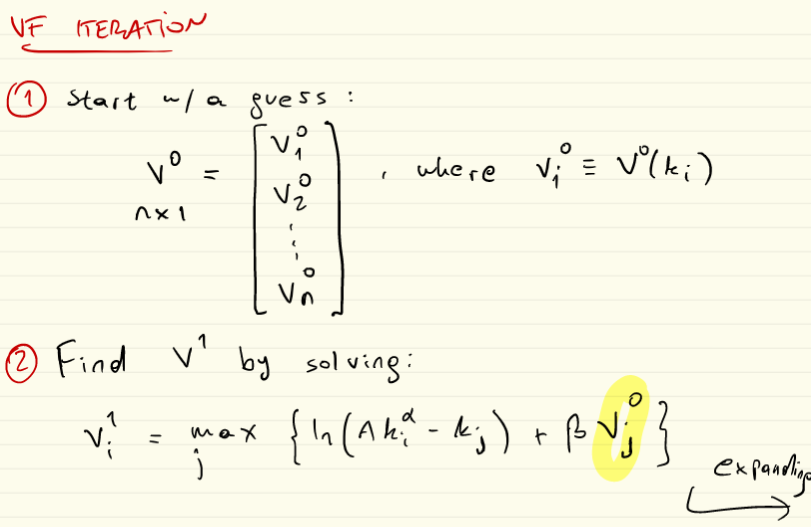
\includegraphics[width=8cm, height=6cm]{pic1}
            \item 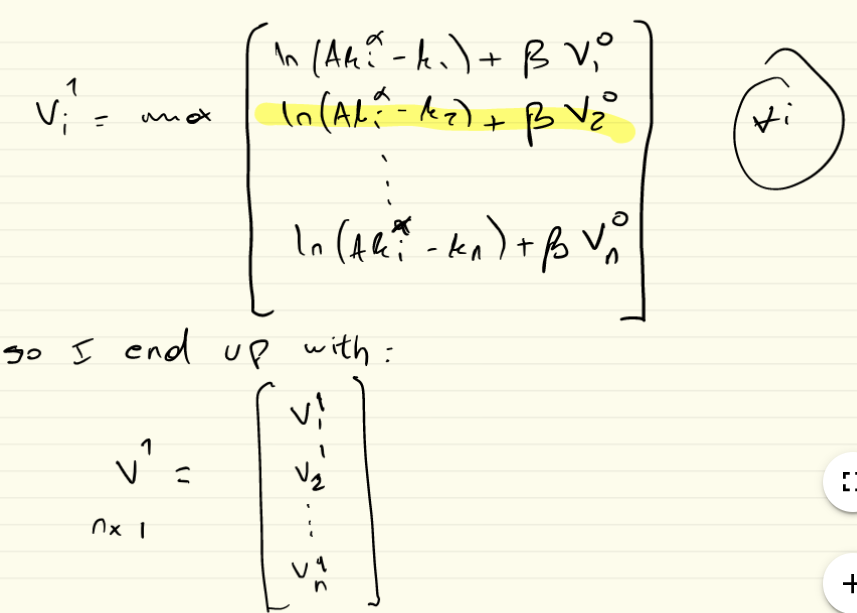
\includegraphics[width=8cm, height=6cm]{pic2}
            \item 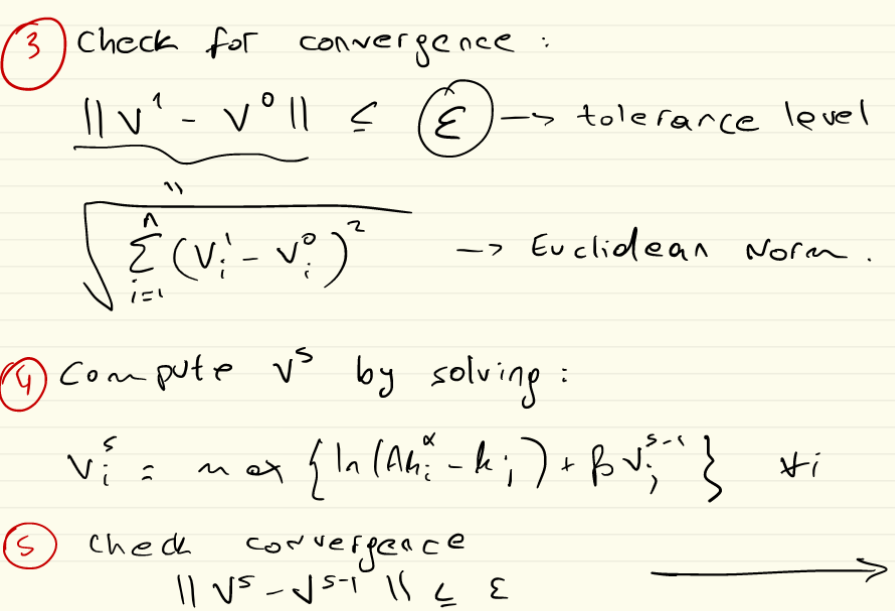
\includegraphics[width=8cm, height=6cm]{pic3}
            \item 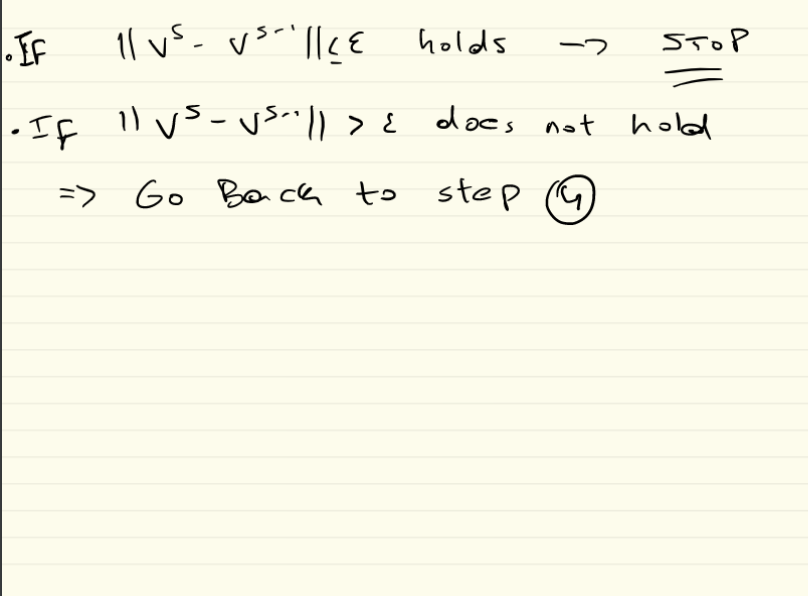
\includegraphics[width=8cm, height=6cm]{pic4}
        \end{itemize}
    \end{itemize}
\end{itemize}
\vspace{2.5mm}
\par \underline{\bf{Ordinary Differential Equations (ODEs)}}: a "differential" equation" is one where the unknown is a function (instead of a variable) and the equation includes one or more of the derivatives of the function, an "ordinary differential equation" equation is one for which the unknown is a function of only one variable (typically time)
\begin{itemize}
    \item \underline{Partial ODEs}: where the unknown is a function of more than one variable
    \item  \underline{First-Order ODE Form}: $\dot{x}(t) = F(t, x(t))$, where $\dot{x}(t) \equiv dx(t)/dt$ and $t \in [t_{a}, t_{b}]$
    \begin{itemize}
        \item \underline{Unknown}: here the unknown is a function $x(t)$ with $x: [t_{a}, t_{b}] \rightarrow \mathbb{R}$
        \item  \underline{Uniqueness}: the solution is not unique with the form having infinitely many solutions indexed by an integrating constant C. However, generally the constant C can be uniquely determined by requiring the solution to pass through a given point on the $tx$-plane
        \item  \underline{Example}: $\dot{x}(t) = 2t$ with $t \in [0,\infty)$
        \begin{itemize}
            \item \underline{Solution without Initial Condition}: the general solution is $x(t) = t^{2} + C$
            \item  \underline{Solution with Initial Condition}: suppose we impose the initial condition $x(0) = 1$, therefore $C=1$ and the particular solution is $x(t) t^{2} + 1$
            \item 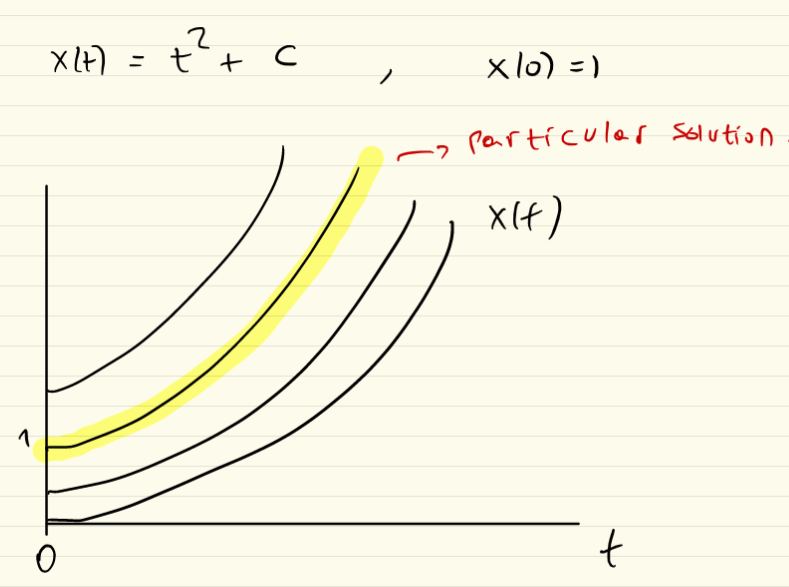
\includegraphics[width=8cm, height=6cm]{pic5}
        \end{itemize}
    \end{itemize}
    \item  \underline{Finite-Difference Methods for Solution}: here we approximate derivates using finite-differences to approximate the solution to the ODE. This involves finding $\dot{x}(t) = F(t,x(t))$, $x(t_{a}) = x_{a}$, and $t \in [t_{a}, t_{b}]$. There are a wide range of methods depending on how the derivatives are approximated
    \begin{itemize}
        \item  \underline{Euler's Method}
        \begin{itemize}
            \item  \underline{Step 1}: specify a grid for t, i.e. $t_{0} = t_{a} < t_{1} < t_{2} < \dots < t_{N} = t_{b}$
            \item  \underline{Step 2}: approximate the ODE using the difference equation $$\tfrac{x(t_{i+1}) - x(t_{i})}{t_{i+1}-t_{i}} = F(t_{i},x(t_{i}))$$ over $i = 0, \dots, N-1$, where $x(t_{0})=x_{a}$ is fixed by the initial condition
            \item  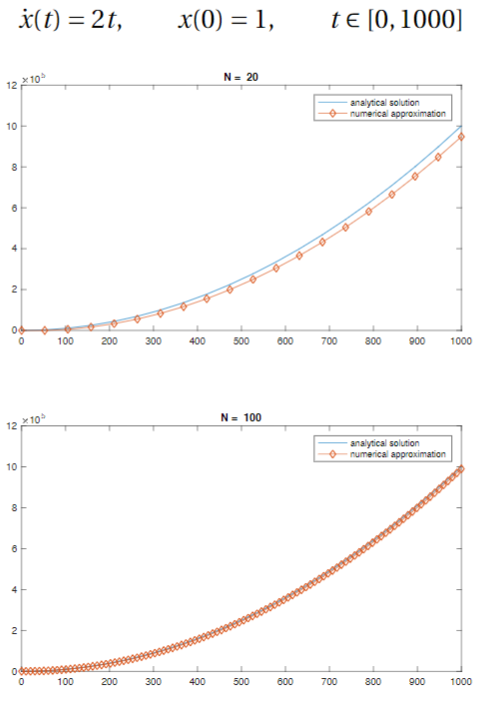
\includegraphics[width=8cm, height=6cm]{pic6}
            \item  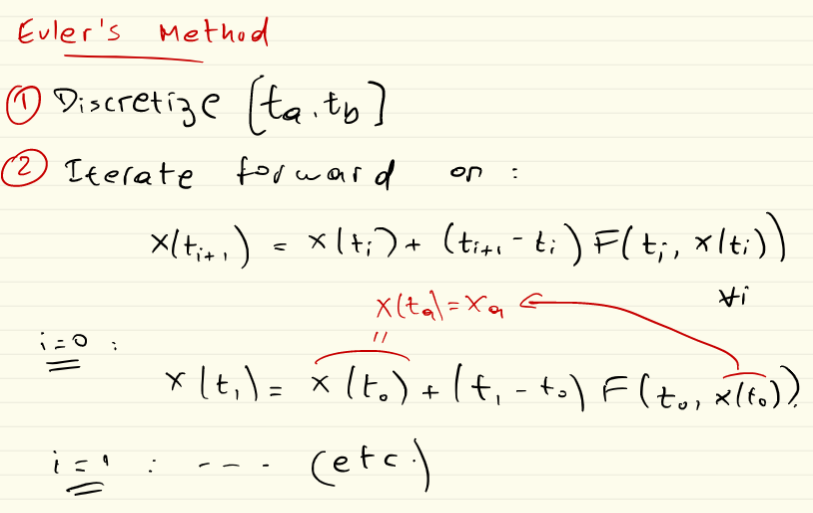
\includegraphics[width=8cm, height=6cm]{pic7}
        \end{itemize}
    \end{itemize}
    \item \underline{ODE Systems}: consider the system of two equations in two unknowns
    \begin{gather*}\dot{x}(t) = f(t, x(t), y(t)) \\ \dot{y}(t) = g(t, x(t), y(t)) \end{gather*} where $t \in [t_{a}, t_{b}]$. The general solution typically depends on two arbitrary constants,  say A and B, and can be written as \begin{gather*} x(t) = \phi_{1} (t; A, B) \\ y(t) = \phi_{2} (t; A,B) \end{gather*} Here A and B can be pinned down via two conditions on the solution and two types of problems emerge depending on the nature of such conditions. Note that, like single-equation ODEs, exact solutions to ODE systems can only be obtained under special cases
    \begin{itemize}
        \item \underline{Initial Value Problem(IVP)}: $x(t_{a}) = x_{a}$, $y(t_{a}) = y_{a}$, can be solved numerically by applying Euler's Methods
        \begin{itemize}
            \item \underline{Step 1}: discretize the domain
            \item  \underline{Step 2}: iterate forward starting from $x(t_{a}) = x_{a}$ and $y(t_{a}) = y_{a}$
        \end{itemize}
        \item  \underline{Boundary Value Problem (BVP)}: $x(t_{a}) = x_{a}$, $y(t_{b}) = y_{b}$, can be solved by applying a shooting algorithm
        \begin{itemize}
            \item \underline{Step 1}: make an initial guess for $y(t_{a})$ called $y_{a}^{G}$
            \item \underline{Step 2}: solve the ODE system by applying Euler's method given $x(t_{a}) = x_{a}$ and $y(t_{a}) = y_{a}^{G}$
            \item \underline{Step 3}: if $y(t_{b})$ is 'close enough' to $y_{b}$ then stop, else update $y_{a}^{G}$ and go back to step 2
            \item 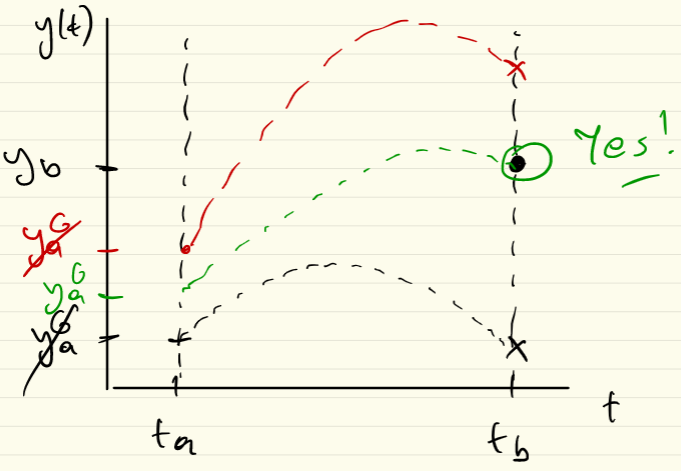
\includegraphics[width=8cm, height=6cm]{pic8}
        \end{itemize}
    \end{itemize}
    \item \underline{Higher-Order ODEs}: techniques for solving ODE systems also apply to analysing higher-order Equations
    \begin{itemize}
        \item \underline{Example}: consider the second-order ODE \begin{gather*} \ddot{x}(t) = f(t, \dot(t), x(t)) \end{gather*} where $\ddot{x}(t) \equiv \partial^{2}x(t) / \partial t^{2}$.
        Define the new variables $y = \dot{x}$ and you are left with the two-equation ODE system
        \begin{gather*} \dot{y} (t) = f(t, y(t), x(t)) \\ \dot{x}(t) = y(t) \end{gather*}
    \end{itemize}
\end{itemize}
\vspace{2.5mm}
\par \underline{\bf{The Maximum Principle}}: the typical continuous time optimization problem is
\begin{gather*} \max_{x(t), y(t)} \ \int_{0}^{t_{1}} f (t,x(t), y(t)) \ \ \ dt \end{gather*}
subject to
\begin{gather*} \dot{x}(t) = g\big(t, x(t), y(t)\big), \ \ \ x(t) \in \mathcal{X} \ \forall t, \ \ \ y(t) \in \mathcal{Y} \ \forall t, \ \ \ x(0) = x_{0} \end{gather*}
There are two main issues with conventional solution methods to this problem; (1) we are choosing over infinitely dimensional objects such as the function $x: [0, t_{1}] \rightarrow \mathcal{X}$, (2) the constaints include a differential equation rather than a set of equalities/inequalities. In order to overcome these issues and find a solution, we apply the maximum principle theorem
\begin{itemize}
    \item \underline{Notation and Assumptions}: $x$ is the state variable, $y$ is the control variable, $\mathcal{X} \subset \mathbb{R}$  and $\mathcal{Y} \subset \mathbb{R}$ are nonempty and convex, $f$ and $g$ are continuously differentiable in their arguments, we define a Hamiltonian, and for simplicity we assume $t_{1} < \infty$
    \begin{itemize}
        \item  \underline{Hamiltonian}: we define the hamiltonian $$H(t,x(t),y(t),\mu(t)) \equiv f(t,x(t),y(t)) + \mu(t)g(t,x(t),y(t))$$ where $\mu(t)$ is a continuously differentiable function called the costate variable
    \end{itemize}
    \item  \underline{Maximum Principle Theorem}: suppose that the aforementioned continuous time problem has an interior continuous solution $(\widehat{x}(t), \widehat{y}(t))$. Then there exists a continuously differentiable function $\mu(t)$ such that
    \begin{gather*} H_{y}(t,\widehat{x}(t), \widehat{y}(t), \mu(t)) = 0 \ \forall t \in [0, t_{1}] \\ \dot{\mu}(t) = -H_{x}(t, \widehat{x}(t), \widehat{y}(t), \mu(t)) \ \forall t \in [0, t_{1}] \\ \mu(t_{1}) = 0 \end{gather*}
    \begin{itemize}
        \item \underline{ODE Usage}: by $H_{y}(t,\widehat{x}(t), \widehat{y}(t), \mu(t)) = 0$ we can write $y = Y(t, x \mu)$. Using $\dot{\mu}(t) = -H_{x}(t, \widehat{x}(t), \widehat{y}(t), \mu(t))$ and $mu(t_{1}) = 0$ and combining the law of motion we are left with
        \begin{gather*} \dot{x} = g\big(t, x, Y(t,x,\mu)\big) \\ \dot{\mu} = -H_{x}\big(t,x,Y(t,x,\mu),\mu \big) \\ x(0) = x_{0}, \ \ \ \mu(t_{1}) = 0 \end{gather*}
        which is an ODE system in $x$ and $\mu$ that can be solved numerically by applying the shooting algorithm
        \item \underline{Sufficient Condition Requirements}: the maximum principle only provides necessary conditions for an optimum, sufficient conditions for a maximum rely on concavity properties of the objective and on convexity of the feasible set
        \item \underline{Technique Generalization}: the techniques generalize to multidimensional problems (where $x$ and $y$ are vectors), infinite horizon problems (ie $t_{1} = \infty$), and to including terminal conditions on the final state (e.g. $x(t_{1}) = x_{1}$)
        \item \underline{Index}: the variable t may represent time or any other index
    \end{itemize}
\end{itemize}

\end{document}
